\chapter{Introduction}
\section{Plasma}
Plasma is often called the fourth state of matter after solid, liquid, and gas. \cite{chen_introduction_2016} In a plasma, the atoms or molecules have been stripped of electrons, resulting in a collection of charged particles, ions and electrons.

\begin{figure}[htbp]
	\centering
	\includegraphics[width=0.7\textwidth]{figures/plasma-properties}
	\caption{Typical plasmas. Adapted from \cite{cpep_physics}}
	\label{fig:plasma-properties}
\end{figure}

Plasma is a common state of matter. We can find on Fig.\ref{fig:plasma-properties}, examples of natural plasma include nebula, stars, sun, etc. We are able to see entire galaxies in the sky because they are in plasma state, and plasma is capable of emitting light. \cite{chen_introduction_2016} Artificially generated plasma can be found in fluorescent lights, Neon signs, fusion reactors. These plasmas have different densities and temperatures.

Plasma has various scientific and technological uses. It is used in plasma physics research, nuclear fusion experiments, plasma cutting and welding, plasma medicine for treating diseases, and even in spacecraft propulsion systems.

Overall, plasma is an intriguing and versatile state of matter with significant implications in various fields of science, technology, and industry.

\subsection{Single Particle Motion Along Magnetic Field Line}
Plasma consists of charged particles, and is governed by electromagnetic force. Assume magnetic field only, the particle motion is governed by Lorentz force and the particles will gyrate along the magnetic field lines. The equation of motion of a charged particle in magnetic field is given by
\[ m\dv{\mathbf{v}_p}{t} = q\mathbf{v}_p\times \mathbf{B} \]
where $m$ is the mass of charged particle, $q$ is the charge of particles, and $\mathbf{v}_p$ is the velocity of the particle.

Consider a magnetic field pointing in z-direction, $\mathbf{B}=B\mathbf{\hat{z}}$. Since the magnetic force is perpendicular to both $\mathbf{v}_p$ and $\mathbf{B}$, we can separate the equation of motion into two directions,
\[
	q\mathbf{v_{\perp}\times B} = \frac{mv_{\perp}^2}{r}\mathbf{\hat{r}},
	\quad
	\mathbf{v}_{\parallel} = v_{\parallel} \mathbf{\hat{z}} \]
where $\mathbf{v}_{\perp}$ is the velocity perpendicular to the magnetic field, and $\mathbf{v}_{\parallel}$ is the velocity parallel to the magnetic field, and $\mathbf{\hat{r}}$ is a unit vector pointing from the central axis of the helical motion to the trajectory of the particle. In this way, we see that the charged particle is doing circular motion in the plane of $\mathbf{\hat{r}}$, gyrating along the magnetic field line with Larmor radius $r$ and Larmor frequency $\omega_c = \abs{q}B/m$. On the other hand, the particle is flowing freely in the direction of $\mathbf{B}$ since there is no force in this direction. The charged particle is doing helical motion along the magnetic field line.

\subsection{Adiabatic Invariants}
The charged particles always travel on the same magnetic field line in the magnetic nozzle. To show this we will introduce two adiabatic invariants.

\subsubsection*{Magnetic Moment}
In classical mechanics, the action integral $\oint pdq$ taken over a period of a periodic motion is a constant. Here $p$ and $q$ are generalized momentum and coordinate. In single particle motion along magnetic field line, one obvious periodic motion is the Larmor gyration. Take $p$ to be the angular momentum $mv_\perp r$ and $q$ to be the angular coordinate $\theta$, the action integral becomes

\begin{equation}
	\oint pdq = \oint mv_\perp r_L d\theta = 2\pi r_L mv_\perp = 2\pi \frac{mv_\perp^2}{\omega_c} = 4\pi\frac{m}{\abs{q}}\left(\frac{mv_\perp^2}{2B}\right)
\end{equation}

Define the quantity magnetic moment as

\begin{equation}
	\mu = \frac{mv_\perp^2}{2B}
\end{equation}

We see that the magnetic moment $\mu$ is constant as long as $q/m$ is constant.

\subsubsection*{Longitudinal Invariant}
The next adiabatic invariant is the quantity defined as \cite{chen_introduction_2016}
\begin{equation}
	J=\int_a^b v_\parallel ds
\end{equation}
where $a$ and $b$ are the two turning points in magnetic mirror, see Fig.\ref{fig:particle-in-mirror}.

\begin{figure}[htbp]
	\centering
	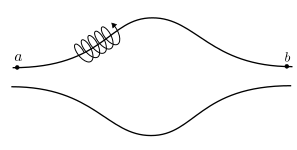
\includegraphics[width=0.7\textwidth]{figures/particle-in-mirror.png}
	\caption{A particle bouncing between turning points $a$ and $b$ in a magnetic field. Adapted from \cite{chen_introduction_2016}.}
	\label{fig:particle-in-mirror}
\end{figure}

Since the particle's energy is conserved and is equal to $mv_\perp^2/2$ at the turning point, the invariance of $\mu$ indicates that $\abs{B}$ remains the same at the turning point. However, upon drifting back to the same longitude, a particle may find itself on another line of force at a different altitude. This cannot happen if $J$ is conserved. $J$ determines the length of the line of force between turning points, and no two lines have the same length between points with the same $\abs{B}$. Consequently, the particle returns to the same line of force even in a slightly asymmetric field.


\begin{figure}[htbp]
	\centering
	\includegraphics[width=0.7\linewidth]{figures/gyrate-along-b-field}
	\caption{A charged particle gyrates about the magnetic field line. The velocity along the field line is $\mathbf{v}_{\parallel}$ and the gyrate frequency, radius is given by the radial equation, $q\mathbf{v_{\perp}\times B} = \mathbf{\hat{r}} mv_\perp^2/r$. Moreover, for static, nonuniform magnetic field, the charged particle will stay on the same of magnetic field line as it gyrates.}
	\label{fig:gyrate-along-b-field}
\end{figure}

\subsection{From Kinetic Theory to Fluid Description}
Although the previous treatment is useful for single particle, to describe the collective behavior of a large amount of particles, we need to do that in the framework of kinetic theory. In kinetic theory, the charged particles in plasma obey a certain distribution function,
\[f(\mathbf{x}, \mathbf{v}_p, t)\]
It describes the probability density at position $\mathbf{x}$ with velocity $\mathbf{v}$ at time $t$.

Suppose a collisionless plasma in 3-dimensional space is at thermal equilibrium, then the particles can be characterized by Maxwell-Boltzmann distribution
\[ f_M(\mathbf{x}, \mathbf{v}_p, t) = \frac{n(\mathbf{x}, t)}{(\pi v_{th}^2)^{3/2}} \exp(-\left(\frac{v}{v_{th}}\right)^2) \]
where $n(\mathbf{x},t)$ is number density of the particles, $v_{th} = \sqrt{2k_BT/m}$ is the thermal velocity, and $v=\sqrt{v_x^2+v_y^2+v_z^2}$.

The moments of the distribution function are suitable macroscopic properties of the plasma. For example, the plasma number density and momentum can be viewed as

\[ n(\mathbf{x}, t) = \int_{\mathbb{R}^3} f(\mathbf{x}, \mathbf{v}_p, t) d^3\mathbf{v}_p \]
\[ n\mathbf{v}(\mathbf{x}, t) = \int_{\mathbb{R}^3} \mathbf{v}_p f(\mathbf{x}, \mathbf{v}_p, t) d^3\mathbf{v}_p \]
where $\mathbf{v}$ is the fluid velocity of the charged particle. It is the bulk velocity of the plasma. The charged particles flow along the magnetic field line, it is intuitive to think of $\mathbf{v}$ as the plasma flow velocity along the magnetic field line.

In this thesis we assume collisionless plasma. The distribution function $f$ in a collisionless plasma satisfies the so-called collisionless Vlasov equation, $\dv*{t} f(\mathbf{x}, \mathbf{v}, t) = 0$. Expand it explicitly, it is
\begin{equation} \label{eq:vlasov}
	\pdv{f}{t} + \mathbf{v}\pdv{f}{\mathbf{x}} + \frac{q}{m}(\mathbf{E} + \mathbf{v}\times\mathbf{B})\pdv{f}{\mathbf{v}} = 0
\end{equation}
where $q(\mathbf{E} + \mathbf{v}\times\mathbf{B})$ is the Lorentz force experience by the species, the collision term $C(f)$ is dropped.

Integrate both sides with respect to volume element in velocity space, $d^3\mathbf{v}$, we get the conservation of density.
\[ \pdv{\rho}{t} + \div(\rho\mathbf{v}) = 0 \]

If we multiply $\mathbf{v}$ on both sides and integrate with respect to $d^3\mathbf{v}$, we get the conservation of momentum.
\[ \rho\pdv{\mathbf{v}}{t} + \mathbf{v}\cdot\grad{\mathbf{v}} = \frac{q}{m}(\mathbf{E+v\times B}) - \grad{p} \]
In the process we assume isotropic pressure, and no viscosity exists in the plasma.

As we can see the fluid description only depends on the macroscopic properties of plasma, such as the fluid velocity along the magnetic field line $\mathbf{v}$, mass density $\rho$, and pressure $p$ of the plasma. This simplifies the problem.

\section{Instability of Plasma Flow}
The instability of plasma flow refers to the tendency of a plasma system to deviate from a stable, equilibrium state and exhibit perturbations or fluctuations in its behavior. It can be understood as the simple mechanical analogy with a ball on crest / in valley. On the left of Fig.\ref{fig:stability-visualization} shows us a stable equilibrium, small perturbations given to the system will not push the ball far away from the equilibrium position, the valley. Hence, the equilibrium is stable. On the right, any small perturbations will cause the ball to fall downhill, hence the equilibrium is unstable. The instabilities in plasma can arise from various factors, such as the interaction of particles with electromagnetic fields, collective effects, or the presence of gradients in plasma parameters. A famous example of instability is the two stream instability. The configuration starts with two oppositely traveling beams of ions and electrons. As time evolves, chaotic behavior develops as shown in Fig.\ref{fig:two-stream-instability}.

\begin{figure}[htbp]
	\centering
	\includegraphics[width=0.7\linewidth]{figures/stability-visualization.png}
	\caption{Mechanical analogy of various types of equilibrium. Adapted from \cite{chen_introduction_2016}}
	\label{fig:stability-visualization}
\end{figure}

\begin{figure}[htbp]
	\centering
	\includegraphics[width=0.7\linewidth]{figures/two-stream-instability}
	\caption{Visualization of two-stream instability in the phase space. (a) Initially the ion and electron flow are in opposite direction. (b) The velocity of both flows start to oscillate. (c) Chaotic behavior occurs. (d) The chaotic behavior continues. \cite{ha_nonlinear_2011}}
	\label{fig:two-stream-instability}
\end{figure}

Magnetic nozzle is one of the most actively researched configurations in plasma propulsion systems, which is being developed for space missions due to their potential for high efficiency and thrust. Understanding and controlling instabilities in the plasma flow within these nozzles is essential for optimizing their performance and achieving efficient propulsion. Investigating instabilities in plasma flow within magnetic nozzles also contributes to our broader understanding of fundamental plasma physics phenomena.


\subsection*{Linear Instability}
In this thesis, we will focus on the so-called linear instability. Meaning that the perturbation grows / decays only in exponential form. The following is a brief description of the process for analyzing linear instability. The detail treatment will be given in Chap.\ref{chap:theoretical-analysis}.

\begin{enumerate}
	\item State equations of motion: The linear instability analysis starts from the equations of motion which describes the plasma system. In this thesis, the equations of motion are time-dependent fluid equations involving the number density $n$ and velocity $v$ of the plasma flow along the central axis of the nozzle.
	\item Give perturbations to the system: Suppose the system has an equilibrium state $n_0$ and $v_0$. The system will be given small perturbations, they serve as small deviations on number density and velocity, $\tilde{n}$ and $\tilde{v}$. All variables $n$ and $v$ in the equations of motion will be substituted by perturbed quantities, $n_0+\tilde{n}$ and $v_0+\tilde{v}$.
	\item Linearize equations of motion: Expand the equations of motion, and discard the second and higher order terms, often called nonlinear terms, such as $\tilde{n}\tilde{v}$, $\tilde{n}\partial_z\tilde{v}$, $\tilde{v}\partial_z\tilde{n}$ and etc. We obtain the so-called linearized equations of motion. These equations contain only the linear terms.
	\item Assume perturbation takes exponential form: Let perturbations take the form $\exp(-i\omega t)$. This indicates that the perturbations are oscillating with frequency $\omega$ in time. Any time derivative in the linearized equations of motion simply becomes $\partial_t = -i\omega$. Now we obtain equations involving perturbations, $\tilde{n}$ and $\tilde{v}$, and their spatial derivatives, and $\omega$.
	\item Analyze the possible values of $\omega$: The oscillation frequency $\omega$ could be a complex number. If the imaginary part of the temporal frequency is greater than zero, i.e. $\Im(\omega) > 0$, then the system is unstable. This is because the perturbation grows exponentially $\exp(\Im(\omega)t)$ in time. On the other hand, if the imaginary part of the temporal frequency is less than or equal to zero, $\Im(\omega) \leq 0$, then the system is said to be stable. Since the perturbations will not be growing, $\Im(\omega)=0$, or even damped, $\Im(\omega) < 0$.
\end{enumerate}

In the later chapters, we devoted much effort to analyze the temporal frequency $\omega$. We will employ spectral method to analyze the temporal frequency for subsonic and supersonic velocity profiles, and shooting method will be employed to obtain temporal frequency.

\section{Magnetic Nozzle}
In this thesis, we are going to deal with plasma flow in magnetic nozzle.
A magnetic nozzle is a device that uses a magnetic field to shape and control the flow of charged particles in a plasma propulsion system, see Fig.\ref{fig:magnetic-nozzle}. By employing magnetic mirrors, the magnetic nozzle can efficiently direct and accelerate the plasma particles, generating thrust for propulsion. The magnetic field in the nozzle helps collimate and focus the plasma exhaust, increasing its velocity and enhancing the performance of the propulsion system.

\begin{figure}[htbp]
	\centering
	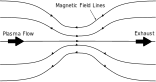
\includegraphics[width=0.7\linewidth]{figures/magnetic-nozzle.png}
	\caption{A simplified example of a magnetic nozzle configuration. On the left ($z=-1$) is the entrance of the nozzle. The plasma flows into the nozzle from the left and will be accelerated and finally exhaust through the exit on the right ($z=1$). The magnetic field lines are shaped in such a way that it forms a magnetic mirror configuration. Plasma flow with specific subsonic speed at the entrance will be accelerated to supersonic speed.}
	\label{fig:magnetic-nozzle}
\end{figure}

\subsection{Magnetic Field in Magnetic Nozzle} \label{sec:magnetic-field-in-nozzle}
The magnetic nozzle by its nature is 3-dimensional. We assume the magnetic field is axis-symmetric, then the radial magnetic field and axial magnetic field are constraint by divergence-free condition,
\begin{equation}
	\div\mathbf{B} = \frac{1}{r}\pdv{(rB_r)}{r} + \pdv{B_z}{z} = 0
	\label{eq:divergence-free-condition}
\end{equation}
Since we are interested in the plasma flow near the central axis of the nozzle, paraxial approximation is taken. Meaning that we take the derivative along the magnetic field line $\nabla_\parallel = \pdv*{z}$ when near the central axis. Hence, in this thesis we will treat the flow in magnetic nozzle as a 1-dimensional problem. The axial magnetic field along the central axis is modeled as
\begin{equation}
	B_z(z) = B_0 \left[1 + R\exp(-\left(\frac{z}{\delta}\right)^2)\right], \quad -1\leq z \leq 1
\end{equation}
where $1+R$ is the magnetic mirror ratio, it is the ratio of the magnitude of magnetic field at the center of the nozzle to that at the end of the nozzle, $1+R = B(0)/B(1)$. The mirror ratio $R$ controls the spread of the plasma flow at the exit. On the other hand, $\delta$ determines the spread of the magnetic field. Larger the $\delta$, flatter the magnetic field. An example of magnetic field is shown in Fig.(\ref{fig:magnetic-field}).

The radial profile of magnetic field, $B_r$, is given by the divergence-free condition, Eq.(\ref{eq:divergence-free-condition}). In this thesis will focus on the axial magnetic field only.

\begin{figure}[htbp]
	\centering
	\includegraphics[width=0.7\linewidth]{figures/magnetic-field}
	\caption{This is the magnetic field in nozzle with mirror ratio $1+R=B_{max}/B_{min}=2.5$, and the spread of magnetic field, $\delta=0.1/0.3=0.\bar{3}$. }
	\label{fig:magnetic-field}
\end{figure}

\subsection{Velocity Profiles of Plasma Flow in Magnetic Nozzle}
The analytical solution gives 4 different kinds of velocity profiles,
\begin{itemize}
	\item Subsonic profile: Plasma flow enters and exits the nozzle with subsonic speed. Every point on this profile is subsonic.
	\item Supersonic profile: Plasma flow enters and exits the nozzle with supersonic speed. Every point on this profile is supersonic.
	\item Accelerating profile: Plasma flow enters the nozzle with subsonic speed and exits the nozzle with supersonic speed. Points before the nozzle throat are subsonic, and the flow reaches ion sound speed at the nozzle throat, then the flow is supersonic after the nozzle throat.
	\item Decelerating profile: Plasma flow enters the nozzle with supersonic speed and exits the nozzle with subsonic speed. Similar to the accelerating profile, but the velocity is decreasing.
\end{itemize}
See Fig.\ref{fig:velocity-profiles} for these profiles.

The velocity of plasma flow in the magnetic nozzle is given by the Lambert W function, Eq.(\ref{eq:velocity-profile}). The Lambert W function has 2 different branches, corresponding to the subsonic and supersonic branches in the velocity profiles. The expression of velocity profile will be derived in Chap.\ref{chap:theoretical-analysis}.

\section{Flow in Similar Configuration: Bondi-Parker Flow}
Consider a massive celestial object in the space. This celestial object will attract matter in the space because it is massive. Hence, creating an accretion flow. If the celestial object is a star, it can also eject matter into space. Solar wind is an example to this since it is a stream of charged particles, primarily electrons and protons, flowing outward from the Sun. Bondi derived a steady-state solution for accretion flow which is governed by Bernoulli's equation in spherical symmetry around a point mass in 1952. Hence, the inward accretion flow is also called Bondi flow. Then Parker solved a similar problem but with outward wind in 1958. Then the outward wind is given the name, Parker flow. \cite{aikawa_stability_1979,bondi_spherically_1952,keto_stability_2020} The Bondi and Parker flow (also called Bondi-Parker flow) is similar to that in magnetic nozzle. It is interesting to compare the two configurations.

\subsection{Governing Equations and Velocity Profiles}
The governing equations for one-dimensional, spherically symmetric, stationary isothermal flow neglecting self-gravity are \cite{velli_hydrodynamics_2001},
\begin{align*} \label{eq:bondi-parker}
	\pdv{r}(\rho vr^2) = 0, \quad p = c^\rho \\
	v\pdv{v}{r} = -\frac{1}{\rho}\pdv{p}{r} - \frac{GM}{r^2}
\end{align*}
where $v,\rho,p$ are velocity, density, pressure, $c$ the constant sound speed, $M$ the mass of the star or other central object, and $GM/r^2$ the gravitational acceleration. For a static atmosphere, the pressure profile is given by $p=p_0\exp(-g/c^2 + g/rc^2)$. In terms of mach number $M=v/c$ the flow equations may be written as
\[ \left(M - \frac{1}{M}\right)M' = \frac{2}{r} - \frac{g}{r^2c^2} \]

It has a singular point at the sonic point, $r=\frac{g}{2c^2}, M=1$. The equilibrium velocity profiles in such configuration are shown in Fig.\ref{fig:BP-flow-velocity}. For the transonic flow in magnetic nozzle, there also exists a singularity and it is located at the throat of the nozzle, $z=0$, we will illustrate this in Chap.\ref{chap:singular-perturbation}.

If we compare the velocity profiles for Bondi-Parker flow and the flow in magnetic nozzle. We found they are similar. The flow in magnetic nozzle can also be grouped into three different types: subsonic, supersonic, and transonic. See Fig.\ref{fig:velocity-profiles}. For subsonic profiles, every point on the curve is slower than sound speed. While every point on the supersonic velocity profile is faster than sound speed. Lastly, there are two different transonic profiles: accelerating profile and decelerating profile. The accelerating profile describes the accelerating plasma flow which is at subsonic speed at the entrance of the nozzle and is accelerated to supersonic speed at the exit of the nozzle. The decelerating profile is similar.

\begin{figure}[htbp]
	\centering
	\includegraphics[width=0.7\textwidth]{figures/steady-state-BP-flow}
	\caption{Representative trajectories of the steady-state BP flow in non-dimensional units. \cite{keto_stability_2020} The upward pink line represents an outward wind, it accelerates from subsonic to supersonic. The downward pink line represents an accretion flow, it accelerates towards the mass point. The green lines below the pink lines represent subsonic flows, and the green lines above represent supersonic flows. Orange lines are physically impossible scenarios.}
	\label{fig:BP-flow-velocity}
\end{figure}

\subsection{The Stability of Bondi-Parker Flow}
In this subsection we will focus our attention to the outgoing flow because it is similar to the flow in magnetic nozzle. In the research \cite{velli_from_1994,del_dynamical_1998} of instabilities of Bondi-Parker flow, they are using Dirichlet boundary conditions, meaning that the perturbation is 0 at the surface of the celestial object and at infinity.

Under such boundary conditions, the decelerating outflow solution for Bondi-Parker flow is physically impossible because it is unstable. Moreover, the subsonic breeze is also unstable due the unfavorable stratification. Last but not least, the supersonic shocked wind and transonic flow are stable. \cite{velli_hydrodynamics_2001}

In our research, all types of flows but decelerating flow are stable.

\section{Goals of this Thesis}
Fusion is considered the next-generation source of a clean, safe and abundant energy providing an opportunity to address climate change problems. A new high-tech industry has appeared in the last decade fueled by over \$4 billion of private investments, with the second world largest and several other smaller companies founded in Canada. To achieve controlled fusion, one of the key science problems is to understand and learn to predict the non-linear behavior of plasma due to waves and instabilities. The general objective of my research is to understand the behavior and learn to control the turbulent flows of plasmas in magnetically controlled fusion system, in particular, open magnetic mirrors. I study the instabilities of the flow in a magnetic mirror configuration under different boundary conditions which is an open question and is under debate in application to fusion systems and also related to the solar wind flows.

The general objective of this research is to understand the stability of the flow in a magnetic nozzle. Plasma confined by the magnetic field is typically far from the state of the thermodynamic equilibrium which makes it unstable. In this project, we would like to investigate the stability of plasma flow in a magnetic nozzle under different boundary conditions. Understanding the instabilities of plasma flow in a magnetic mirror configuration is important in applications such as the expanding magnetic divertors in controlled fusion and electric propulsion. \cite{ryutov_divertor_2016,kaganovich_2020_physics}

In the following thesis, fluid model of plasma will be reviewed and linearized governing equations will be derived in chapter \ref{chap:theoretical-analysis}. The problem will be then formulated as an eigenvalue problem. In chapter \ref{chap:spectral-method}, spectral method and shooting method for solving eigenvalue problem will be introduced. In the section of spectral method, different discretizations of the operators, such as finite difference and spectral method will be discussed. Moreover, spectral pollution and its filtering will as also be investigated. Then in the next section, we will formulate the problem to the form suitable for applying shooting method. We will apply both shooting method and spectral method to the problem. By comparing the results from two different methods, the credibility of the results are increased. In chapter \ref{chap:numerical-experiments}, we will use the method developed in chapter \ref{chap:spectral-method} to conduct numerical experiments. The goal is to extract the eigenvalues (frequency) of each oscillating mode. Conclusion will in chapter \ref{chap:discussion}.
